% Plantilla del artículo del Proyecto Integrador (Resumen ejecutivo)
% Formato requerido: carta, una columna, 11 pt, márgenes de 2.5 cm, interlineado 1.15.
% Extensión: 3 páginas sin contar anexos. Referencias: APA 7.
% Compila con pdfLaTeX (opción predeterminada de Overleaf) + Biber.
% Logos: logo.jpeg (Tec) y logo_empresa.png (empresa) en la misma carpeta.
% Si un archivo no existe, se muestra un recuadro de marcador.
\documentclass[letterpaper,11pt]{article}

\usepackage[utf8]{inputenc}
\usepackage[T1]{fontenc}
\usepackage{lmodern}
\usepackage[spanish,es-tabla,es-nodecimaldot]{babel}
\usepackage[margin=2.5cm]{geometry}
\usepackage{setspace}
\setstretch{1.15}
\usepackage{graphicx}
\usepackage{booktabs}
\usepackage[font=small,labelfont=bf]{caption}
\usepackage{csquotes}
\usepackage[hidelinks]{hyperref}

% Estilo de referencias: APA 7
\usepackage[style=apa,backend=biber]{biblatex}
\addbibresource{referencias2.bib}

% --- Complementos del resumen ejecutivo ---
\usepackage{xcolor}
\setlength{\parindent}{1.5em}

% --- Encabezado: logos solo en la primera página ---
\usepackage{fancyhdr}
\geometry{headheight=52pt,headsep=0.3cm}
\renewcommand{\headrulewidth}{0pt}
\newcommand{\logo}[2]{%
  \IfFileExists{#1}%
    {\includegraphics[height=1.2cm]{#1}}%
    {\fbox{\parbox[c][1.1cm][c]{3cm}{\centering\sffamily\small #2}}}}
\fancypagestyle{primera}{%
  \fancyhf{}%
  \fancyhead[L]{\logo{logo.jpeg}{Logo Tec}}%
  \fancyhead[R]{\logo{logo_unam.png}{Logo empresa}}%
  \fancyfoot[C]{\thepage}}
\pagestyle{fancy}
\fancyhf{}
\fancyfoot[C]{\thepage}

% --- Recuadros de cifras (texto grande) ---
% \cifra{fondo}{color del texto}{valor}{etiqueta}{unidad}
\newcommand{\cifra}[5]{%
  \begingroup\setlength{\fboxsep}{5pt}%
  \colorbox{#1}{\parbox[t]{\dimexpr\linewidth-2\fboxsep\relax}{%
    \setstretch{1}\color{#2}{\Large\bfseries #3}\par
    #4%
    \ifx\relax#5\relax\else\par{\footnotesize #5}\fi}}%
  \endgroup}
\newcommand{\cifragris}[4]{\cifra{black!8}{black}{#1}{#2}{#3}}
\newcommand{\cifraacento}[4]{\cifra{blue!10}{blue!55!black}{#1}{#2}{#3}}

% --- Complementos de tablas y figuras ---
\usepackage{amsmath}
\usepackage{array}
\usepackage{tabularx}
\usepackage{float}
\newcolumntype{Y}{>{\raggedright\arraybackslash}X}
\graphicspath{{figuras/}}

\begin{document}
\thispagestyle{primera}

% --- Título y datos ---
\noindent{\LARGE\bfseries Clasificacion morfologica de galaxias mediante fusion multimodal de imagenes DESI Legacy y espectros integrados MaNGA\par}
\smallskip
\noindent{\large\textcolor{black!60}{Resumen ejecutivo para el Instituto de Astronomía de la UNAM}\par}
\medskip

\noindent\begingroup\setlength{\fboxsep}{6pt}%
\colorbox{black!8}{\parbox{\dimexpr\linewidth-2\fboxsep\relax}{\small\setstretch{1.05}%
\textcolor{black!60}{Integrantes:} Alexander Carreño, Julio R. Velázquez, María Rabelero\\
\textcolor{black!60}{Programa:} Proyecto Integrador · Maestría en Inteligencia Artificial Aplicada\\
\textcolor{black!60}{Asesores:} Dr. José A. Vázquez Mata y Dr. Héctor M. Hernández Toledo \textcolor{black!60}{Fecha:} Noviembre de 2026}}%
\endgroup\par\medskip

% --- Problema y solución ---
La clasificación morfológica de galaxias se realiza principalmente mediante inspección visual; a gran escala consume tiempo especializado y puede variar entre clasificadores. El reto crecerá con los grandes volúmenes de imágenes del Vera C. Rubin Observatory (LSST), cuya explotación científica requiere métodos reproducibles y escalables. Galaxy Vision explora una clasificación binaria inicial —galaxias tempranas (Ttype $\leq 0$) y tardías (Ttype $\geq 1$)— combinando imágenes, espectros MaNGA y poblaciones estelares STARLIGHT. La propuesta es usar el modelo como apoyo para priorizar y organizar la revisión científica, no como sustituto del criterio experto.\

El Instituto de Astronomía de la UNAM clasifica la morfología de las galaxias por inspección visual. El proceso es lento, depende del criterio de cada persona y no escalable. El Observatorio Vera C. Rubin generará cerca de 20TB de imágenes por noche durante diez años \parencite{ivezic2019}. \emph{Galaxy Vision} automatiza el primer filtro: un modelo de visión por computadora, entrenado con 9,351 galaxias de MaNGA etiquetadas por los expertos del patrocinador \parencite{bundy2015, vazquezmata2022}, lee la imagen a color del DESI Legacy Survey \parencite{dey2019} e indica en segundos si la galaxia es \emph{temprana} (elíptica o lenticular) o \emph{tardía} (espiral o irregular), con un nivel de confianza. Las galaxias claras se clasifican solas y las dudosas pasan a revisión experta.

% --- Cifras de desempeño del modelo ---
\medskip
\noindent
\begin{minipage}[t]{0.235\linewidth}\cifraacento{0.967}{AUC}{separa clases (máx.~1)}{}\end{minipage}\hfill
\begin{minipage}[t]{0.235\linewidth}\cifragris{89.5\,\%}{Exactitud}{+6.6 pp sobre la meta}{}\end{minipage}\hfill
\begin{minipage}[t]{0.235\linewidth}\cifragris{89.8\,\%}{{\small Exactitud balanceada}}{90.9\,\% / 88.7\,\% por clase}{}\end{minipage}\hfill
\begin{minipage}[t]{0.235\linewidth}\cifragris{0.014}{Error de calibración}{confianza fiable (ideal~0)}{}\end{minipage}
\medskip

% --- Desempeño ---
En 1,403 galaxias que nunca vio, el modelo acierta 9 de cada 10 de forma equilibrada en ambas clases, supera la meta de exactitud (82.9\,\%), al modelo de referencia ResNet-18 (88.8\,\%) y a las variantes con espectros o poblaciones estelares, que no aportaron mejora demostrable (Figura~\ref{fig:desempeno}a); las cifras coinciden con el artículo del proyecto \parencite{carreno2026}. Como su confianza está bien calibrada, sirve para decidir qué revisar: con el umbral fijado en validación, el 82\,\% de las galaxias se clasifica sola con 94.9\,\% de exactitud y solo el 18\,\% va a un experto (Figura~\ref{fig:desempeno}b). Elegir el punto operativo por su costo de revisión lo vuelve rentable \parencite{baccarin2020}. \textbf{El desempeño es suficiente para producción con revisión humana de casos inciertos}, no como sustituto de la etiqueta científica.

\begin{figure}[!t]
\centering
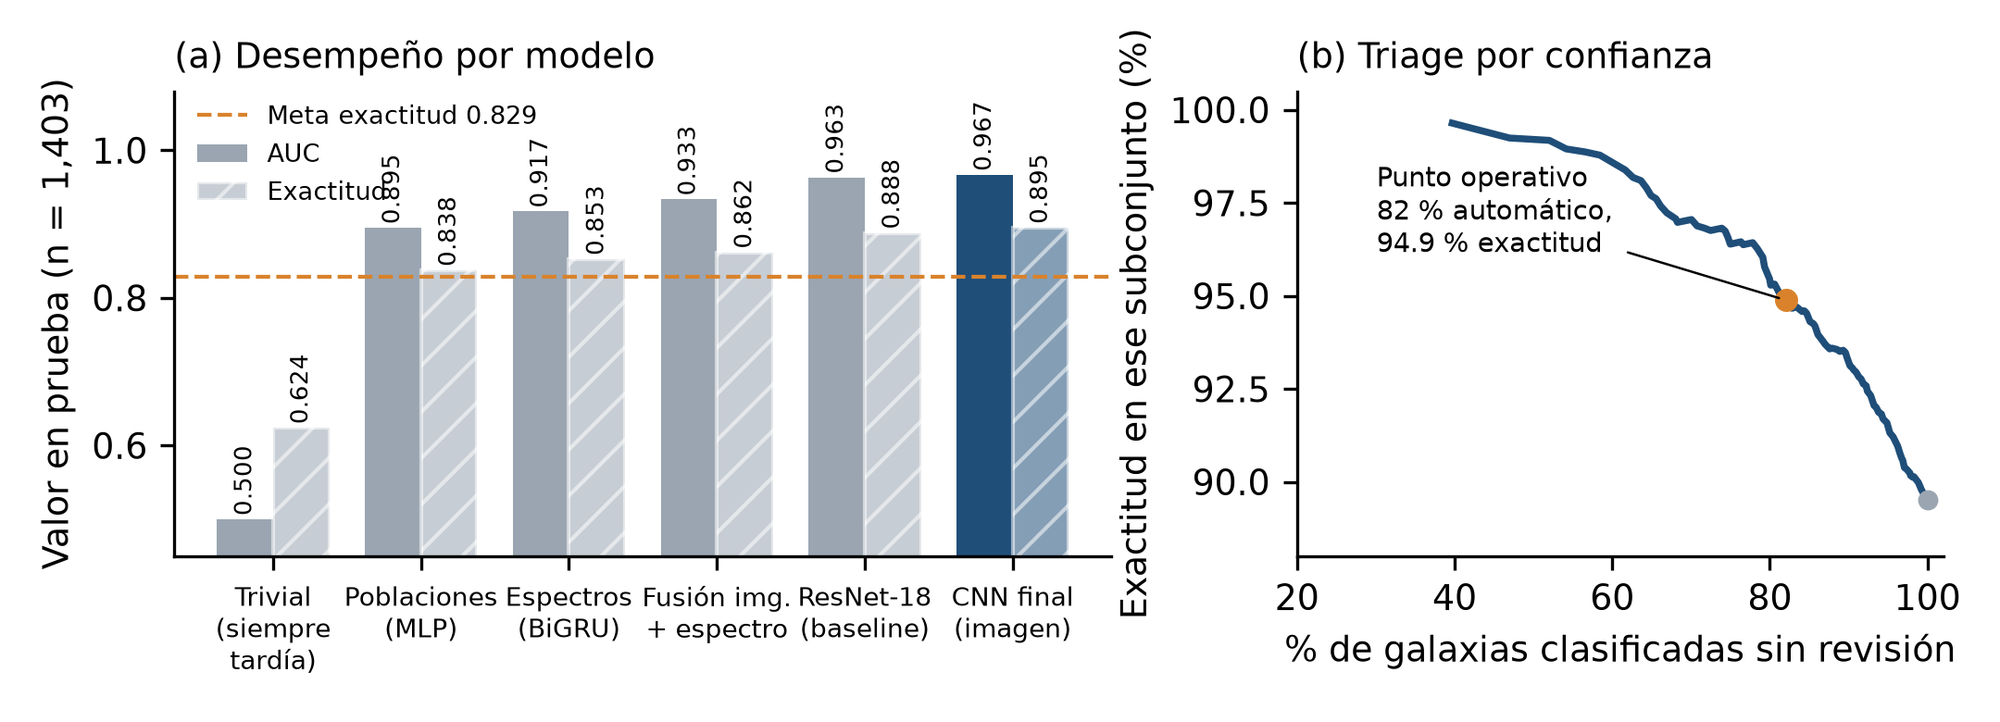
\includegraphics[width=\linewidth]{fig1_desempeno.png}
\vspace{-16pt}
\caption{(a) AUC y exactitud en prueba de los modelos evaluados frente a la meta. (b) Exactitud del modelo final al clasificar automáticamente solo las galaxias de mayor confianza; el punto naranja es el umbral propuesto.}
\label{fig:desempeno}
\end{figure}

% --- Beneficios cuantificables (mensuales) ---
\medskip
\noindent Para 10,000 galaxias al mes, 1.5 minutos de experto por galaxia y \$350~MXN por hora-experto, los beneficios mensuales estimados son:

\smallskip
\noindent
\begin{minipage}[t]{0.235\linewidth}\cifragris{$-$201\,h}{Ahorro de tiempo}{horas/mes ($-$80\,\%)}{}\end{minipage}\hfill
\begin{minipage}[t]{0.235\linewidth}\cifragris{$-$\$70.3\,mil}{Costos operativos}{MXN/mes}{}\end{minipage}\hfill
\begin{minipage}[t]{0.235\linewidth}\cifragris{$-$60\,\%}{Reducción de errores}{628 errores menos/mes}{}\end{minipage}\hfill
\begin{minipage}[t]{0.235\linewidth}\cifragris{+409\,\%}{Capacidad}{de 40 a 204 gal./hora-experto}{}\end{minipage}

\smallskip
\noindent{\footnotesize\textcolor{black!60}{Cálculo y supuestos en el Anexo~A. El ahorro supone revisar solo el 18\,\% dudoso más una auditoría del 2\,\%; los errores se comparan contra clasificar todo sin revisión.}}
\medskip

\noindent\textbf{Mejora en la toma de decisiones.} Una probabilidad calibrada por galaxia permite priorizar y dimensionar la revisión con datos.
\textbf{Mejora en la calidad.} Un criterio único y versionado reduce la variabilidad entre clasificadores.
\textbf{Simplificación del trabajo.} Los expertos dejan los casos obvios y se enfocan en los ambiguos o interesantes.
\textbf{Diferenciación competitiva.} El IA-UNAM llega a Rubin/LSST con una herramienta propia y publicable.
\medskip

% --- Inversión y costos (TCO a 12 meses) ---
El costo total de propiedad (TCO) a 12 meses suma desarrollo, tres meses de implementación y nueve de operación en la nube, dominada por mantenimiento más que por cómputo (desglose en el Anexo~B).

\smallskip
\noindent
\begin{minipage}[t]{0.235\linewidth}\cifragris{\$115.5\,mil}{Desarrollo}{MXN, ya ejercido}{}\end{minipage}\hfill
\begin{minipage}[t]{0.235\linewidth}\cifragris{\$87.0\,mil}{Implementación}{MXN, meses 1--3}{}\end{minipage}\hfill
\begin{minipage}[t]{0.235\linewidth}\cifragris{\$88.5\,mil}{Operación}{MXN, meses 4--12}{}\end{minipage}\hfill
\begin{minipage}[t]{0.235\linewidth}\cifraacento{\$291.0\,mil}{TCO 12 meses}{MXN}{}\end{minipage}
\medskip

Con ahorro de \$70.3~mil y operación de \$9.8~mil al mes, la inversión se recupera en el mes 7 y deja un beneficio neto de \$342~mil~MXN el primer año. \textbf{Recomendación:} aprobar \$175.5~mil~MXN adicionales: \$87~mil para implementar ya y \$88.5~mil para operar, liberados en el mes 3 solo si (1) AUC $\geq$0.95 y exactitud $\geq$87\,\% con 5 semillas, (2) $\geq$94\,\% de exactitud en lo automático en un piloto de 1,000 galaxias revisado por expertos y (3) hay un responsable técnico designado en el IA-UNAM.

% --- Riesgos y mitigación ---
\begin{table}[H]
\centering\footnotesize\setstretch{1}
\caption{Principales riesgos de la implementación y su mitigación.}
\label{tab:riesgos}
\vspace{-4pt}
\begin{tabularx}{\linewidth}{@{}>{\raggedright\arraybackslash}p{0.45\linewidth}Y@{}}
\toprule
\textbf{Riesgo} & \textbf{Mitigación}\\
\midrule
\textbf{1. Validez de etiquetas (datos).} La frontera Ttype 0--1 es ambigua: 16.1\,\% de las galaxias y 47.8\,\% de los errores. & El triage envía los casos dudosos a revisión; re-etiquetar 1,000 casos frontera con dos expertos a ciegas y reentrenar (Anexo~C).\\[2pt]
\textbf{2. Deriva de datos (modelo).} Imágenes de Rubin/LSST o FITS difieren de DR11 y el desempeño puede caer sin aviso \parencite{babic2021}. & Monitoreo mensual de confianza y tasa de revisión; validar con muestra etiquetada antes de usar datos nuevos.\\[2pt]
\textbf{3. Robustez no demostrada.} Resultados de una sola semilla y partición. & Repetir con 5 semillas y bootstrap; es condición de la recomendación.\\[2pt]
\textbf{4. Errores con alta confianza.} 22.3\,\% de los errores de imagen escapan al triage. & Auditoría aleatoria del 2\,\% de lo automático y revisión mensual.\\[2pt]
\textbf{5. Continuidad operativa.} Sin servicio desplegado; el conocimiento reside en el equipo. & Contenedor, registro de modelos, guía operativa y capacitación a un responsable.\\
\bottomrule
\end{tabularx}
\end{table}

% --- Transferencia y continuidad ---
\vspace{-14pt}
\section*{Transferencia y continuidad}
\vspace{-6pt}
El IA-UNAM recibirá el repositorio de código (datos, entrenamiento, inferencia y contenedor Docker), los pesos del modelo final con su configuración y métricas, las particiones y el manifiesto de datos para reproducir resultados, las predicciones, los cuadernos, el artículo técnico, dos sesiones de capacitación y una guía operativa para clasificar lotes, ajustar el umbral, monitorear la deriva y reentrenar (Anexo~D).

\vspace{-8pt}
\section*{Declaración de uso de inteligencia artificial}
\vspace{-6pt}
Se utilizó \textcite{anthropic2026claude} para la revisión de redacción, el formato del documento y la generación de gráficas. Los autores verificaron las cifras; la responsabilidad final sobre el contenido recae en ellos.

% --- Referencias ---
\vspace{-8pt}
\renewcommand*{\bibfont}{\small}
\printbibliography[title={Referencias}]

% --- Anexos ---
\clearpage
\section*{Anexo A. Cálculo de beneficios mensuales}
Las cifras de triage se obtuvieron de las predicciones guardadas del modelo final: el umbral de confianza (0.54 en escala $2|p-0.5|$) se fijó en validación para lograr exactitud $\geq$95\,\% en lo automático y se aplicó sin cambios a prueba. El artículo advierte que la reducción de trabajo no se midió en un flujo productivo \parencite{carreno2026}; por ello se presentan como estimaciones a confirmar en el piloto.

\begin{table}[H]
\centering\small
\caption{Supuestos del modelo de beneficios.}
\label{tab:supuestos}
\begin{tabularx}{\linewidth}{@{}p{0.34\linewidth}p{0.15\linewidth}Y@{}}
\toprule
\textbf{Supuesto} & \textbf{Valor} & \textbf{Justificación}\\
\midrule
Volumen a clasificar & 10,000 gal./mes & Equivale al catálogo MaNGA completo en un mes; conservador frente a Rubin/LSST.\\
Tiempo de experto por galaxia & 1.5 min & Inspección de imagen a color y asignación de tipo; un solo clasificador.\\
Costo cargado por hora de experto & \$350 MXN & Investigador o posdoctorante: $\approx$\$56~mil/mes con prestaciones entre 160~h.\\
Fracción automática (cobertura) & 82\,\% & Prueba: 1,152 de 1,403 galaxias sobre el umbral (validación: 81.6\,\%).\\
Exactitud en lo automático & 94.9\,\% & Prueba: 59 errores en 1,152 galaxias (validación: 95.1\,\%).\\
Exactitud sin triage & 89.5\,\% & Exactitud global del modelo final (147 errores en 1,403).\\
Auditoría aleatoria & 2\,\% & Muestra de lo automático revisada por expertos.\\
Revisión experta & corrige el caso & La etiqueta experta es la referencia del proyecto.\\
Tipo de cambio & \$18.5 MXN/USD & Supuesto para convertir precios de nube.\\
\bottomrule
\end{tabularx}
\end{table}

\begin{table}[H]
\centering\small
\caption{Beneficios cuantificables mensuales: valor, unidad y base de cálculo.}
\label{tab:beneficios}
\begin{tabularx}{\linewidth}{@{}p{0.2\linewidth}p{0.17\linewidth}p{0.15\linewidth}Y@{}}
\toprule
\textbf{Indicador} & \textbf{Valor} & \textbf{Unidad} & \textbf{Base de cálculo}\\
\midrule
Ahorro de tiempo & 201 h ($-$80.4\,\%) & horas/mes & Manual: $10{,}000 \times 1.5/60 = 250$~h. Con triage: $10{,}000 \times (0.18 + 0.82 \times 0.02) \times 1.5/60 = 49.1$~h. Ahorro: $250 - 49.1 = 200.9$~h.\\
Ahorro en costos operativos & \$70,315 & MXN/mes & $200.9~\text{h} \times \$350$. Costo de operación de la solución: \$9,834/mes (Anexo~B); ahorro neto \$60,481/mes.\\
Reducción de errores & 628 ($-$59.9\,\%) & errores/mes & Sin triage: $10{,}000 \times 0.1048 = 1{,}048$. Con triage: $8{,}200 \times 0.0512 = 420$ errores no detectados.\\
Incremento en capacidad de procesamiento & +409\,\% & galaxias/ hora-experto & $10{,}000/250 = 40$ frente a $10{,}000/49.1 = 204$ galaxias por hora de experto ($\times$5.09).\\
\bottomrule
\end{tabularx}
\end{table}

\section*{Anexo B. Costo total de propiedad (TCO) a 12 meses}
Horizonte: meses 1--3 de implementación y 4--12 de operación. Costo de operación: \$9,834 MXN al mes. Tarifas por hora: ciencia de datos \$250, ingeniería MLOps \$400, asesoría científica \$600 y experto revisor \$350~MXN. Cómputo: instancia AWS g4dn.xlarge bajo demanda a 0.526~USD/h \parencite{aws2026ec2} y almacenamiento S3 a 0.023~USD/GB-mes \parencite{aws2026s3}.

\begin{table}[H]
\centering\small
\caption{Desglose del TCO por servicio (MXN).}
\label{tab:tco}
\begin{tabularx}{\linewidth}{@{}p{0.17\linewidth}Y r@{}}
\toprule
\textbf{Etapa} & \textbf{Servicio y base de cálculo} & \textbf{MXN}\\
\midrule
Desarrollo & Equipo de ciencia de datos (3 personas × 120 h × \$250) & 90,000\\
 & Asesoría científica IA-UNAM (2 asesores × 20 h × \$600) & 24,000\\
 & Cómputo GPU de experimentación (150 h × \$9.73) & 1,460\\
 & Datos públicos (Legacy Survey, MaNGA, STARLIGHT) & 0\\
\cmidrule(l){2-3}
 & \textit{Subtotal desarrollo} & \textit{115,460}\\
Implementación & Ingeniería MLOps: contenedor, \emph{pipeline}, registro de modelos (160 h × \$400) & 64,000\\
 & Re-etiquetado experto de la banda Ttype 0--1 (1,000 gal. × 2 expertos × 1.5 min × \$350/h) & 17,500\\
 & Validación con 5 semillas y bootstrap (10 h GPU) & 97\\
 & Capacitación y transferencia (2 sesiones × 3 h × 3 instructores × \$300) & 5,400\\
\cmidrule(l){2-3}
 & \textit{Subtotal implementación} & \textit{86,997}\\
Operación & Inferencia GPU (10 h/mes × 9 meses) & 876\\
(9 meses) & Servidor de \emph{pipeline} y monitoreo (CPU, 35 USD/mes) & 5,828\\
 & Almacenamiento de imágenes y artefactos (500 GB) & 1,915\\
 & Mantenimiento y monitoreo (16 h/mes × \$400) & 57,600\\
 & Reentrenamiento trimestral (3 × [8 h × \$400 + 3 h GPU]) & 9,688\\
 & Auditoría de errores de alta confianza (4 h/mes × \$350) & 12,600\\
\cmidrule(l){2-3}
 & \textit{Subtotal operación} & \textit{88,506}\\
\midrule
\multicolumn{2}{@{}l}{\textbf{TCO 12 meses}} & \textbf{290,963}\\
\bottomrule
\end{tabularx}
\end{table}

\begin{figure}[H]
\centering
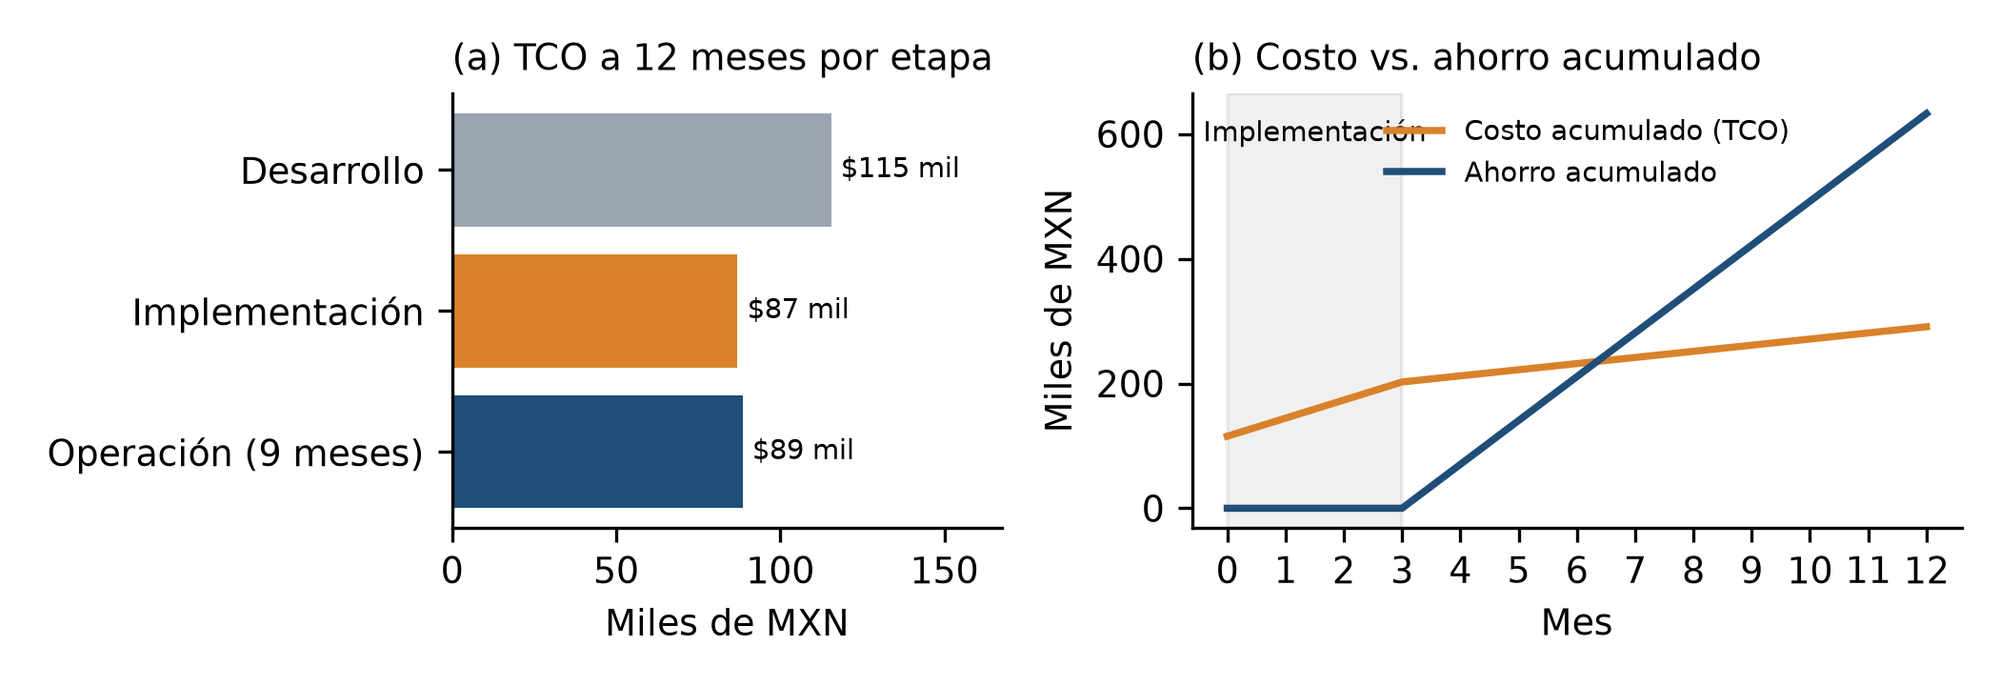
\includegraphics[width=0.95\linewidth]{figA2_tco.png}
\vspace{-8pt}
\caption{(a) TCO por etapa. (b) Costo acumulado frente a ahorro acumulado: el ahorro de 9 meses (\$632.8~mil) supera al TCO en el mes 7 y deja un beneficio neto de \$341.9~mil~MXN.}
\label{fig:tco}
\end{figure}

\section*{Anexo C. Evidencia del riesgo de etiquetas}

\begin{figure}[H]
\centering
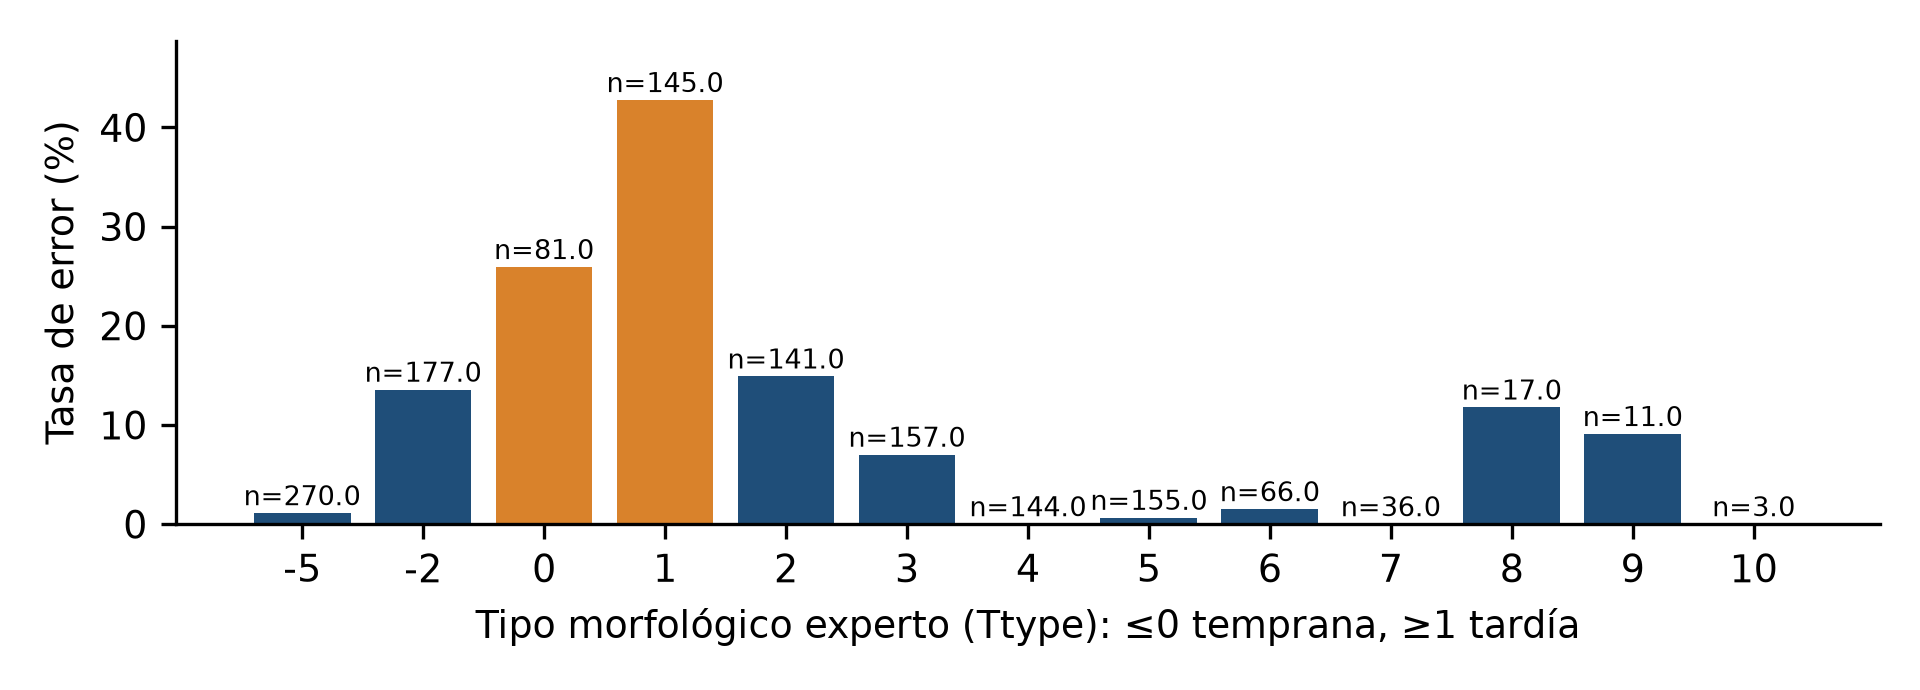
\includegraphics[width=0.72\linewidth]{figA1_error_ttype.png}
\vspace{-8pt}
\caption{Tasa de error del modelo final por tipo morfológico experto en prueba (cálculo propio sobre sus predicciones). La banda Ttype 0--1 (naranja) agrupa 16.1\,\% de las galaxias y 56.5\,\% de sus errores (36.7\,\% de error frente a 5.4\,\% fuera de ella). El artículo reporta 47.8\,\% para el análisis de errores de imagen; ambos confirman la concentración en la frontera (riesgo~1).}
\label{fig:ttype}
\end{figure}

\section*{Anexo D. Entregables y guía operativa}

\begin{table}[H]
\centering\small
\caption{Artefactos que se entregan al IA-UNAM.}
\label{tab:entregables}
\begin{tabularx}{\linewidth}{@{}p{0.3\linewidth}Y@{}}
\toprule
\textbf{Artefacto} & \textbf{Contenido y uso}\\
\midrule
Repositorio de código & Preparación de datos, descarga de imágenes Legacy Survey, entrenamiento, evaluación e inferencia; \texttt{Dockerfile}.\\
Modelo final & Pesos de la CNN (1,222,753 parámetros), \texttt{config.json}, \texttt{history.csv}, \texttt{results.json}.\\
Datos y trazabilidad & Manifiesto de galaxias, particiones con semilla 42, catálogo curado y \texttt{predictions.csv}.\\
Documentación & Artículo técnico, cuadernos de análisis, informe de ablación y este resumen.\\
Guía operativa & Instrucciones paso a paso (abajo), umbrales y responsables.\\
\bottomrule
\end{tabularx}
\end{table}

\noindent\textbf{Guía operativa (resumen).}
\begin{enumerate}\setlength{\itemsep}{0pt}
\item \textbf{Preparar el lote:} generar el manifiesto (\texttt{name}, coordenadas, \texttt{PETRO\_TH90}) y descargar los recortes \emph{grz} de 256×256 píxeles con el campo de visión estándar.
\item \textbf{Clasificar:} ejecutar el contenedor de inferencia con la versión registrada del modelo; la salida guarda identificador, versión, probabilidad, clase y marcas de calidad.
\item \textbf{Enrutar:} las galaxias con confianza $\geq$0.54 pasan al catálogo; el resto, más una muestra aleatoria del 2\,\% de las automáticas, va a la cola de revisión experta.
\item \textbf{Monitorear (mensual):} tasa de revisión (alerta si se aleja más de 5 pp del 18\,\%), exactitud en la auditoría (alerta si $<$94\,\%) y distribución de confianza.
\item \textbf{Reentrenar (trimestral o por alerta):} incorporar etiquetas revisadas en una cohorte versionada, reentrenar con 5 semillas, comparar contra el modelo vigente en una prueba fija y promover solo si no empeora.
\end{enumerate}

\end{document}
```
